\documentclass{article}
\usepackage{geometry}
\usepackage{graphicx}
\usepackage{amsmath}
\usepackage{amssymb}
\usepackage{bm}
\usepackage{xfrac}
\usepackage[utf8]{inputenc}
\usepackage{hyperref}
%
% Format margins
\addtolength{\oddsidemargin}{-.875in}
\addtolength{\evensidemargin}{-.875in}
\addtolength{\textwidth}{1.75in}
\addtolength{\topmargin}{-.875in}
\addtolength{\textheight}{1.75in}
%
% Figure Packages
\usepackage[outercaption]{sidecap}
\usepackage[export]{adjustbox}
\usepackage{graphicx}
\usepackage{caption}
\usepackage{wrapfig}
\usepackage{float}
\usepackage{algorithm, algorithmic, amsfonts,amsmath,amssymb,amsthm, color,comment,enumitem, environ, fancyhdr,   graphicx, mathtools, wasysym}
\pagestyle{fancy}
\setlength{\headheight}{65pt}
\newenvironment{problem}[2][Problem]{\begin{trivlist}
\item[\hskip \labelsep {\bfseries #1}\hskip \labelsep {\bfseries #2.}]}{\end{trivlist}}
\newenvironment{sol}
    {\emph{Solution:}
    }
    {
    \qed
    }
\specialcomment{com}{ \color{blue} \textbf{Comment:} }{\color{black}} %for instructor comments while grading
\NewEnviron{probscore}{\marginpar{ \color{blue} \tiny Problem Score: \BODY \color{black} }}
%%%%%%%%%%%%%%%%%%%%%%%%%%%%%%%%%%%%%%%%%%%%%%%%%%%%%%%%%%%%%%%%%%%%%%%%%%%%%%%%%





%%%%%%%%%%%%%%%%%%%%%%%%%%%%%%%%%%%%%%%%%%%%%
%Fill in the appropriate information below
\lhead{Daniel Agramonte}  %replace with your name
\rhead{MCHE 6390 \\ Homework 3} %replace XYZ with the homework course number, semester (e.g. ``Spring 2019"), and assignment number.
%%%%%%%%%%%%%%%%%%%%%%%%%%%%%%%%%%%%%%%%%%%%%



% Table stuff
\usepackage{multirow}
%\usepackage{floatrow}
%	\floatsetup[table]{capposition=top}%puts table caption above
% Change \subsection title characteristics
    \usepackage[parfill]{parskip}   % forces parskip to not affect headings
    \usepackage{enumitem}           % used for editing itemize environment
    \usepackage{titlesec}
        \titleformat*{\section}{\Large\bfseries\titlerule\vspace{0.5em}}
% Quote blocks
    \usepackage{csquotes} % use environment 'displayquote'
% Create multicolored text commands
    \usepackage[dvipsnames]{xcolor}
        \newcommand{\red}{\color{red}}
        \newcommand{\blue}{\color{blue}}
        \newcommand{\green}{\color{ForestGreen}}
% Misc document settings
    \title{\Huge MCHE 6390 HW03} \author{Daniel Agramonte} \date{09.28.20}
    \setlength{\parindent}{0pt}
    \setlength{\parskip}{1em}
    \setlist{nosep, itemsep=0pt, parsep=0pt}
% Misc vocab commands
    \newcommand{\msalg}{{\fontfamily{cmtt}\selectfont ms83}}
    \newcommand{\lsq}{\emph{lsqnonlin}}
    \newcommand{\msalge}{{\fontfamily{cmtt}\selectfont MCHE\_6500\_NIST\_POLY}}
%
% MATLAB packages
%
\usepackage[framed,numbered]{matlab-prettifier}
\usepackage{textcomp}
\usepackage{xcolor}
\usepackage{listings}
%
% Matrix Spacing
%
\makeatletter
\renewcommand*\env@matrix[1][\arraystretch]{%
  \edef\arraystretch{#1}%
  \hskip -\arraycolsep
  \let\@ifnextchar\new@ifnextchar
  \array{*\c@MaxMatrixCols c}}
\makeatother
%
\begin{document}
\maketitle

\begin{enumerate}
    \item 
    MATLAB code I used to solve the entire problem
    \begin{lstlisting}[style=Matlab-editor]
    % Mass Matrix
    M = [9,0;0,1];
    
    % Stiffness Matrix
    K = [27,-3;-3,3];
    
    %% Part a.
    
    [U,W] = eig(K,M);
    
    N = length(U);
    
    for i = 1:N
        % Mass normalization of modes
        U(:,i) = U(:,i)/sqrt(U(:,i)'*M*U(:,i));
    end
    
    % for some reason MATLAB is liking the negative. It's not technically wrong
    % ,but it's definitely not preferred. Multiplying by -1 bc that's legal.
    
    U = -U;
    
    % Rounds to 4 decimal places
    U = round(U,4);
    
    % U exact
    U_e = [sqrt(2)/6,sqrt(2)/6;sqrt(2)/2,-sqrt(2)/2];
    
    % Rounds to 4 demical places
    U_e = round(U_e,4);
    
    % Error
    eps = U-U_e;
    
    % Max error
    eps_max = max(max(eps));
    
    if eps_max==0
        fprintf('\n\npass!\n\n\n')
    else
        fprintf('\n\nfail\n\n\n')
    end
    
    %% Part b.
    
    % time -> x axis
    t = linspace(0,10,1000);
    
    % r_1
    r_1 = (3*sqrt(2)/2)*cos(sqrt(2)*t);
    
    % r_2
    r_2 = (3*sqrt(2)/2)*cos(2*t);
    
    figure(1)
    
    plot(t,r_1)
    
    hold on
    
    plot(t,r_2)
    
    title('Exact Solution to Example 6.2 in Modal Coordinates')
    xlabel('time [s]')
    ylabel('modal coordinates')
    legend('r_1','r_2')
    
    %% Part c.
    
    % x_1
    x_1 = 0.5*cos(sqrt(2)*t)+0.5*cos(2*t);
    
    % x_2
    x_2 = 1.5*cos(sqrt(2)*t)-1.5*cos(2*t);
    
    figure(2)
    
    plot(t,x_1)
    
    hold on
    
    plot(t,x_2)
    
    title('Exact Solution to Example 6.2 in Physical Coordinates')
    xlabel('time [s]')
    ylabel('Physical Coordinates [m]')
    legend('x_1','x_2')
    \end{lstlisting}
    \begin{enumerate}
        \item
        If the output passes, then there is no difference between the analytic and numeric methods up to 4 digits.
        \begin{lstlisting}[style=Matlab-editor]
        >> MCHE_6390_HW_03_01
        
        
        pass!
        
        
        >> 
        \end{lstlisting}
        The code passed.
        \\
    \newpage
        \item
        Solution in Modal Coordinates
        \begin{figure}[H]
        \vspace{-10pt}
        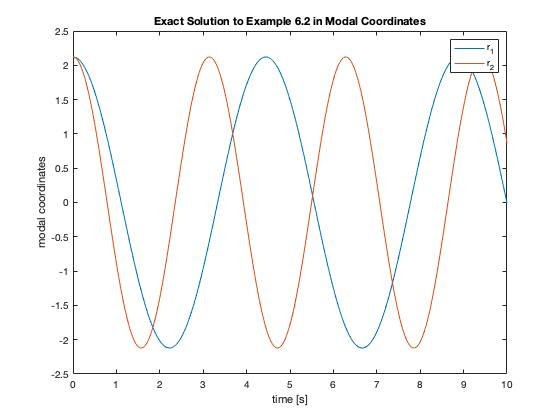
\includegraphics[width=0.7\textwidth,left]{MCHE 6390/HW03/Figures/Figure 1.jpg}
        \label{fig:Modal_Response}
        \end{figure}
        \item
        Solution in Physical Coordinates
        \begin{figure}[H]
        \vspace{-10pt}
        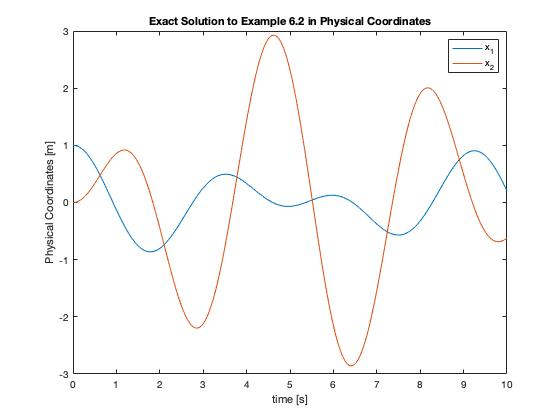
\includegraphics[width=0.7\textwidth,left]{MCHE 6390/HW03/Figures/Figure 2.jpg}
        \label{fig:Physical_Response}
        \end{figure}
    \end{enumerate}
    \newpage
    \item See hand written work
    \item See hand written work
    \item Figures
        \begin{figure}[H]
        \vspace{-10pt}
        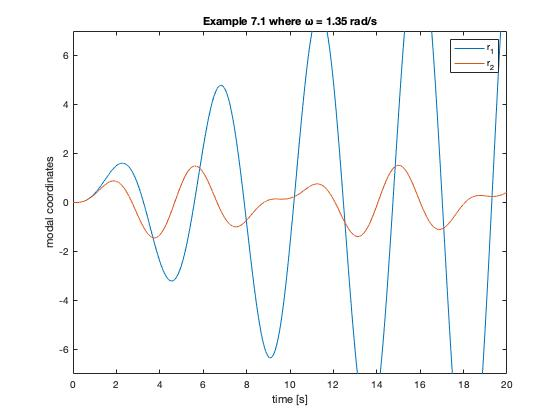
\includegraphics[width=0.7\textwidth,left]{MCHE 6390/HW03/Figures/Figure 3 - 1.35rad.jpg}
        \label{fig:Modal_Response_4_1.35}
        \end{figure}
        
        \begin{figure}[H]
        \vspace{-10pt}
        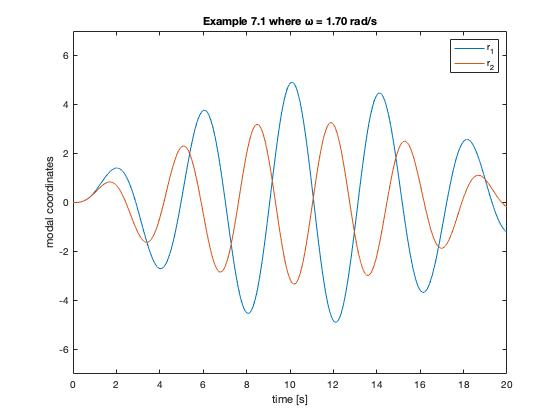
\includegraphics[width=0.7\textwidth,left]{MCHE 6390/HW03/Figures/Figure 3 - 1.70rad.jpg}
        \label{fig:Modal_Response_4_1.70}
        \end{figure}
        
        \begin{figure}[H]
        \vspace{-10pt}
        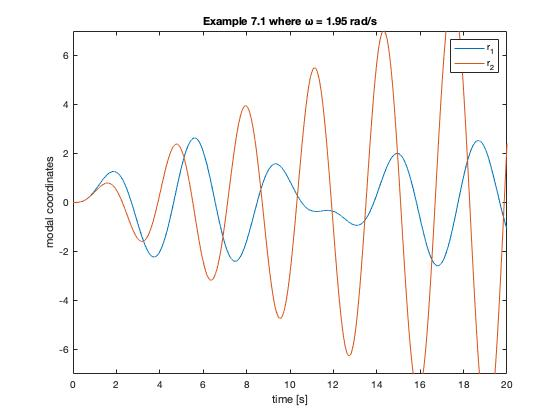
\includegraphics[width=0.7\textwidth,left]{MCHE 6390/HW03/Figures/Figure 3 - 1.95rad.jpg}
        \label{fig:Modal_Response_4_1.95}
        \end{figure}
        
        \begin{figure}[H]
        \vspace{-10pt}
        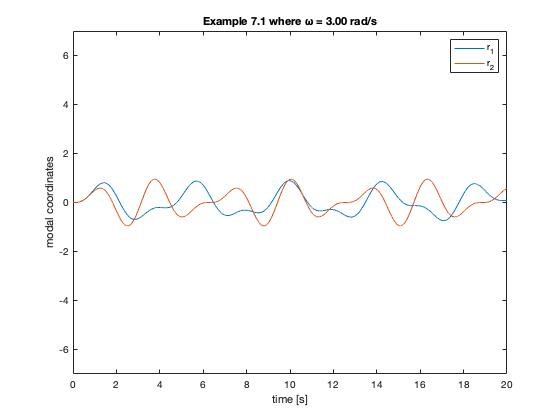
\includegraphics[width=0.7\textwidth,left]{MCHE 6390/HW03/Figures/Figure 3 - 3rad.jpg}
        \label{fig:Modal_Response_4_3}
        \end{figure}
        
        \begin{figure}[H]
        \vspace{-10pt}
        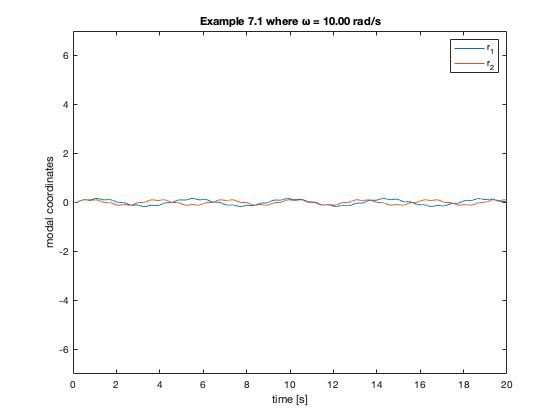
\includegraphics[width=0.7\textwidth,left]{MCHE 6390/HW03/Figures/Figure 3 - 10rad.jpg}
        \label{fig:Modal_Response_4_10}
        \end{figure}
    When $\omega$=1.35 rad/s or $\omega$=1.70 rad/s, there is significant response due to resonance.
    \\
    \\
    MATLAB code I used to solve the entire problem
        \begin{lstlisting}[style=Matlab-editor]
        % Defines w and w_n -> given
        
        w = [1.35,1.7,1.95,3,10];
        wn = [sqrt(2),2];
        
        % time -> x axis
        t = linspace(0,20,10000);
        
        % length of w = 5
        for i = 1:5
            
            % Initializes figure
            figure(i)
            
            % Initializes modal matrix output
            r = zeros(2,10000);
            
            for j = 1:2
                % Solution
                r(j,:) = (2/(wn(j)^2-w(i)^2))*sin(w(i)*t)-(w(i)/wn(j))*...
                    (2/(wn(j)^2-w(i)^2))*sin(wn(j)*t);
                
                plot(t,r(j,:))
                
                % Omega from unicode character list
                omega = char(969);
                
                % Formatting
                ylim([-7,7])
                title(sprintf('Example 7.1 where %s = %.2f rad/s',omega,w(i)))
                xlabel('time [s]')
                ylabel('modal coordinates')
                legend('r_1','r_2')
                
                hold on
            end
        end
        \end{lstlisting}
    \item 
    MATLAB Subroutine
        \begin{lstlisting}[style=Matlab-editor]
            function C = MCHE_6390_HW_03_05(f,m,wn,t)
            
            % Impulse response
            g = @(t,m,wn) (1/(m*wn))*sin(wn*t);
            
            C = integral(@(tau) f(tau).*g(t-tau,m,wn),0,t);
        \end{lstlisting}
    MATLAB Graph Code
        \begin{lstlisting}[style=Matlab-editor]
            % Step Input
            a = @(t) heaviside(t);
            
            % Harmonic Input where omega = 1
            b = @(t) sin(t);
            
            % Intialize domain
            t = linspace(0,10,1000);
            
            % Initialize output vector
            Y = zeros(1000,1);
            Z = zeros(1000,1);
            
            % Set physical parameters to unity
            m = 1;
            wn = 1;
            
            for i = 1:1000
                Y(i) = MCHE_6390_HW_03_05(a,m,wn,t(i));
                Z(i) = MCHE_6390_HW_03_05(b,m,wn,t(i));
            end
            
            figure(1)
            plot(t,Y)
            title('Step Response')
            xlabel('time [s]')
            ylabel('modal coordinates')
            
            figure(2)
            plot(t,Z)
            title('Harmonic Response')
            xlabel('time [s]')
            ylabel('modal coordinates')
        \end{lstlisting}
    \newpage
        Figures 
        
        \begin{figure}[H]
        \vspace{-10pt}
        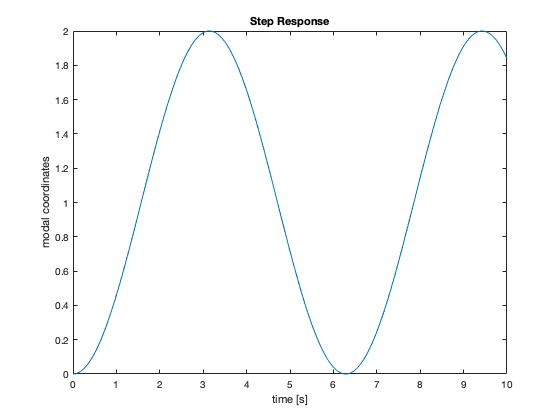
\includegraphics[width=0.7\textwidth,left]{MCHE 6390/HW03/Figures/Figure 4.jpg}
        \label{fig:Step_Response}
        \end{figure}
        
        \begin{figure}[H]
        \vspace{-10pt}
        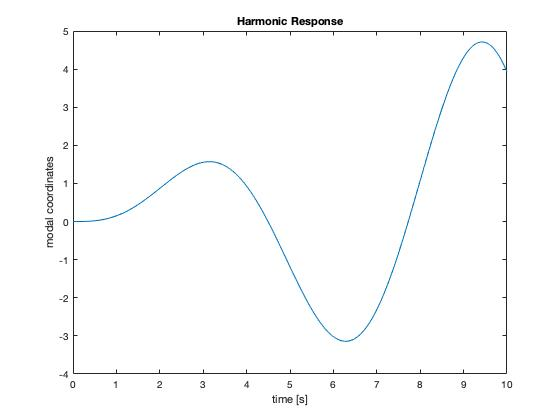
\includegraphics[width=0.7\textwidth,left]{MCHE 6390/HW03/Figures/Figure 5.jpg}
        \label{fig:Harmonic_Response}
        \end{figure}
    \newpage
    \item
    MATLAB Code
        \begin{lstlisting}[style=Matlab-editor]
            % Mass Matrix
            M = eye(3);
            
            % Stiffness Matrix
            K = [4,-2,0;-2,4,-2;0,-2,2];
            
            %% Part a.
            
            [U,W] = eig(K,M);
            
            N = length(U);
            
            for i = 1:N
                % Mass normalization of modes
                U(:,i) = U(:,i)/sqrt(U(:,i)'*M*U(:,i));
            end
            
            % for some reason MATLAB is liking the negative. It's not technically wrong
            % ,but it's definitely not preferred. Multiplying by -1 bc that's legal.
            
            U = -U;
            
            % Modal Influence Matrix - part a
            B_f_a = [2;0;0];
            
            Phi_a = U'*B_f_a;
            
            disp(Phi_a)
            
            %% Part b.
            
            % Modal Influence Matrix - part b
            B_f_b = [1;2;3];
            
            Phi_b = U'*B_f_b;
            
            disp(Phi_b)
            
            %% Part d.
            
            B_f_d = [3;2;3];
            
            Phi_d = U'*B_f_d;
            
            disp(Phi_d)
        \end{lstlisting}
    \newpage
    Solutions:
    \begin{enumerate}
        \item
        \begin{flalign}
            \Phi &=
            \begin{bmatrix}[1.5]
            0.6560\\
            -1.4740\\
            1.1820\\
            \end{bmatrix}&& \nonumber
        \end{flalign}
        \item
            \begin{flalign}
            \Phi &=
            \begin{bmatrix}[1.5]
            3.7209\\
            0.3801\\
            0.1010\\
            \end{bmatrix}&& \nonumber
        \end{flalign}
        \item
        Comparing the $\Phi$ from (a) and (b) we can see that for (b) they are all in phase whereas in (a) $\phi_2$ will be out of phase with $\phi_1$ and $\phi_3$. We can additionally see that for (b), that the magnitude of $\phi_1$ is significantly higher than the other two excited excited modes whereas for (a), the magnitude of excitation is much more even.
        \item
            \begin{flalign}
            \Phi &=
            \begin{bmatrix}[1.5]
            4.3769\\
            -1.0939\\
            1.2830\\
            \end{bmatrix}&& \nonumber
        \end{flalign}
    \end{enumerate}
\end{enumerate}



\end{document}
